\documentclass[letterpaper,11pt]{article}

\usepackage[utf8]{inputenc}
\usepackage{latexsym}
\usepackage[empty]{fullpage}
\usepackage{titlesec}
\usepackage{marvosym}
\usepackage[usenames,dvipsnames]{color}
\usepackage{verbatim}
\usepackage{enumitem}
\usepackage[hidelinks]{hyperref}
\usepackage{fancyhdr}
\usepackage[english]{babel}
\usepackage{tabularx}
\usepackage{tikz}
\usepackage{pgfplots}
\pgfplotsset{compat=1.18}
\input{glyphtounicode}

\usepackage[default]{sourcesanspro}

\pagestyle{fancy}
\fancyhf{}
\fancyfoot{}
\renewcommand{\headrulewidth}{0pt}
\renewcommand{\footrulewidth}{0pt}

\addtolength{\oddsidemargin}{-0.5in}
\addtolength{\evensidemargin}{-0.5in}
\addtolength{\textwidth}{1in}
\addtolength{\topmargin}{-.5in}
\addtolength{\textheight}{1.0in}

\urlstyle{same}
\raggedbottom
\raggedright
\setlength{\tabcolsep}{0in}

\titleformat{\section}{\vspace{-4pt}\scshape\raggedright\large}{}{0em}{}[\color{black}\titlerule \vspace{-5pt}]

\pdfgentounicode=1

\newcommand{\resumeItem}[1]{\item\small{{#1 \vspace{-2pt}}}}
\newcommand{\resumeSubheading}[4]{\vspace{-2pt}\item\begin{tabular*}{0.97\textwidth}[t]{l@{\extracolsep{\fill}}r}\textbf{#1} & #2 \\ \textit{\small#3} & \textit{\small #4} \\ \end{tabular*}\vspace{-7pt}}
\newcommand{\resumeProjectHeading}[2]{\item\begin{tabular*}{0.97\textwidth}{l@{\extracolsep{\fill}}r}\small#1 & #2 \\ \end{tabular*}\vspace{-7pt}}
\newcommand{\resumeSubHeadingListStart}{\begin{itemize}[leftmargin=0.15in, label={}]}
\newcommand{\resumeSubHeadingListEnd}{\end{itemize}}
\newcommand{\resumeItemListStart}{\begin{itemize}}
\newcommand{\resumeItemListEnd}{\end{itemize}\vspace{-5pt}}

\begin{document}

\begin{center}
\textbf{\Huge \scshape Kylian Mbappé} \\ \vspace{1pt}
\small World-Class Forward $|$ Elite Goal Scorer $|$ Manchester United Target Applicant
\end{center}

\section{Professional Summary}
Dynamic and world-renowned professional attacker with an elite track record of high-volume scoring and playmaking. Seeking to leverage exceptional speed, technical precision, and tactical intelligence to lead the Manchester United attacking line. Proven performer in high-pressure environments, consistently delivering match-winning contributions in domestic and international competitions.

\section{Experience}
\resumeSubHeadingListStart
\resumeSubheading{Real Madrid}{2024 -- Present}{Main Attacker}{Madrid, Spain}
\resumeItemListStart
\resumeItem{Serving as the primary attacking focal point, utilizing world-class speed to break defensive lines.}
\resumeItem{Maintaining high conversion rates in La Liga and UEFA Champions League fixtures.}
\resumeItemListEnd

\resumeSubheading{Paris Saint-Germain (PSG)}{2017 -- 2024}{Main Attacker}{Paris, France}
\resumeItemListStart
\resumeItem{Achieved record-breaking goal contributions, becoming the club's all-time leading scorer.}
\resumeItem{Led the team to multiple Ligue 1 titles, consistently delivering 30+ goal involvements per season.}
\resumeItemListEnd
\resumeSubHeadingListEnd

\section{International Career}
\resumeSubHeadingListStart
\resumeSubheading{France National Team}{2017 -- Present}{Forward}{International}
\resumeItemListStart
\resumeItem{FIFA World Cup Champion (2018) and Golden Boot winner (2022).}
\resumeItem{Captain of the national squad, providing leadership and offensive output on the global stage.}
\resumeItemListEnd
\resumeSubHeadingListEnd

\section{Performance Analytics}
\begin{center}
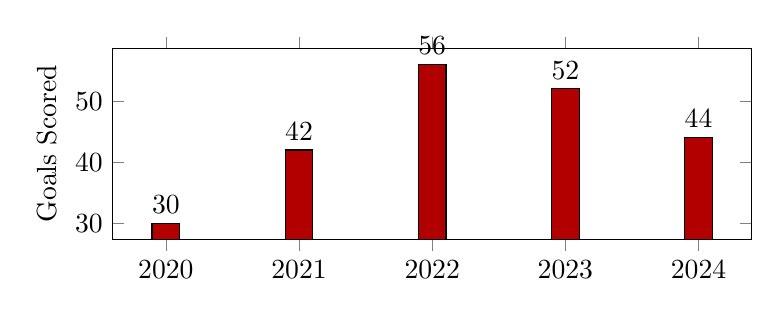
\begin{tikzpicture}
\begin{axis}[
    width=0.8\textwidth, height=4cm,
    ybar, ylabel={Goals Scored},
    symbolic x coords={2020, 2021, 2022, 2023, 2024},
    xtick=data, nodes near coords
]
\addplot[fill=red!70!black] coordinates {(2020,30) (2021,42) (2022,56) (2023,52) (2024,44)};
\end{axis}
\end{tikzpicture}
\end{center}

\section{Technical Skills}
\begin{itemize}[leftmargin=0.15in, label={}]
\item{
\textbf{Offensive Skills}{: Clinical Finishing, Elite Sprint Speed, Tactical Positioning, Dribbling} \\
\textbf{Strategic Capabilities}{: High-Pressing, Playmaking, Set-piece Execution, Game Intelligence} \\
\textbf{Professional Attributes}{: Leadership, High-Pressure Resilience, Adaptability, Team Synergy}
}
\end{itemize}

\section{Awards \& Achievements}
\resumeSubHeadingListStart
\resumeItem{FIFA World Cup Winner (2018), Runner-up (2022)}
\resumeItem{Ligue 1 Player of the Year (Multiple)}
\resumeItem{UEFA Champions League Team of the Season}
\resumeSubHeadingListEnd

\end{document}